\documentclass[11pt,a4paper]{report}

% Language setting
% Replace `english' with e.g. `spanish' to change the document language
\usepackage[portuges]{babel}
% Set page size and margins
% Replace `letterpaper' with `a4paper' for UK/EU standard size
\usepackage[utf8]{inputenc}
\usepackage{graphicx}
\usepackage{url}
\usepackage{enumerate}
\usepackage{color}
\usepackage{multirow}
\usepackage{array}
\usepackage[pdftex]{hyperref}
\usepackage{listings}
\usepackage{enumitem}
\definecolor{codegreen}{rgb}{0,0.6,0}
\definecolor{codegray}{rgb}{0.5,0.5,0.5}
\definecolor{codepurple}{rgb}{0.58,0,0.82}
\definecolor{backcolour}{rgb}{0.95,0.95,0.92}

\lstdefinestyle{mystyle}{
    backgroundcolor=\color{backcolour},   
    commentstyle=\color{magenta},
    keywordstyle=\color{codegreen},
    numberstyle=\tiny\color{codegray},
    stringstyle=\color{codepurple},
    basicstyle=\ttfamily\footnotesize,
    breakatwhitespace=false,         
    breaklines=true,                 
    keepspaces=true,                 
    numbers=left,                    
    numbersep=2pt,                  
    showspaces=false,                
    showstringspaces=false,
    showtabs=true
}

\lstset{style=mystyle}

\title{PLC - Trabalho Prático 2\\
    \large Grupo nº14}

\author{Simão Pedro Batista Caridade Quintela \\ (A97444) 
        \and David José de Sousa Machado \\ (A91665)
        \and Hugo Filipe de Sá Rocha \\ (A96463)
       } %autores do documento
       
\date{\today} %data

\begin{document}

    \begin{minipage}{0.9\linewidth}
        \centering
        
\includegraphics[width=0.4\textwidth]{um.jpg}\par\vspace{1 cm}
        \href{https://www.uminho.pt/PT}
        {\scshape\LARGE Universidade do Minho} \par
        \vspace{0.6cm}
        \href{https://lcc.di.uminho.pt}
        {\scshape\Large Licenciatura em Ciências da Computação} \par
        \maketitle
        
        
\includegraphics[width=0.3\linewidth]{simao.jpg}
        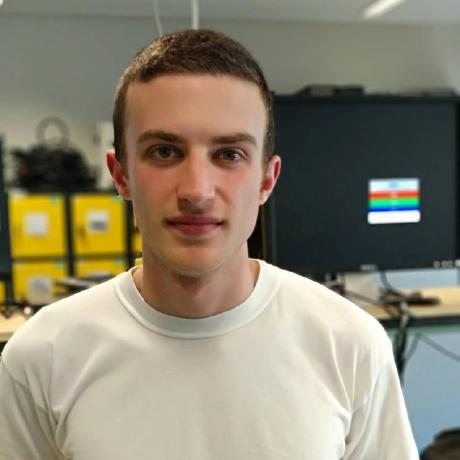
\includegraphics[width=0.3\linewidth]{david.jpg}    
        
\includegraphics[width=0.35\linewidth]{hugo.jpg}
        
        
    \end{minipage}
    
    \tableofcontents
    
    \pagebreak
    
    \chapter{Introdução}
% 
    \paragraph{}
    No âmbito da disciplina de Processamento de Linguagens e Compiladores foi-nos proposto pelo docente Pedro Rangel Henriques o desenvolvimento de uma Linguagem de Programação Imperativa simples e de um compilador para reconhecer programas escritas nessa linguagem gerando o respetivo código Assembly da Máquina Virtual VM.
    \paragraph{}
    Começamos por tentar encontrar um nome original e atrativo para a nossa linguagem e acabou por nos surgir a ideia de colocar o nome "Python-Like-C" cuja sigla (PLC) coincide com a sigla da Unidade Curricular que integra este trabalho (Processamento de Linguagens e Compiladores).
    

    \paragraph{}
    Neste documento está apresentada a gramática da nossa linguagem, o código escrito no módulo Lexer e Yacc do Python e ainda, como foi pedido, alguns testes com código escrito na nossa linguagem e o respetivo código Assembly gerado.

    \chapter{Explicação da nossa linguagem}
    \paragraph{}
    A nossa linguagem contempla os seguintes mecanismos:
    \section{Declaração de variáveis}
    \begin{lstlisting}[language=Python]
    
       int x = 10
       int x
       int x = 10
       int x[n]
       int x[n][m]
    \end{lstlisting}
    \section{Operadores de comparação}
    \begin{lstlisting}[language=Python]
    
       x <= y
       x >= y
       x < y
       x < y
       x == y
    \end{lstlisting}
    \section{Operações numéricas}
    \begin{lstlisting}[language=Python]
    
      x + y
      x - y
      x / y
      x * y
      x % y
      x ++ #(incremento)
      y -- #(decremento)
    \end{lstlisting}
      \section{Operadores lógicos}
    \begin{lstlisting}[language=Python]
    
      x and y
      x or y
    \end{lstlisting}
    \section{Instruções condicionais}
    \begin{lstlisting}[language=Python]
    
     if (cond):
     elif (cond):
     else:
     \end{lstlisting}
     \section{Ciclo do-while}
     \begin{lstlisting}[language=Python]
    
     do:
     ...
     ...
     while(cond):
     \end{lstlisting}
    \section{Input/Output}
    \begin{lstlisting}[language=Python]
    
     x = input()
     x = input("Declare the variable with the value: ")
     print("Hello world!")
     \end{lstlisting}
    \section{Comentário}
    \begin{lstlisting}[language=Python]

     #isto e um comentario na nossa linguagem
     \end{lstlisting}
     

    \chapter{Resolução}
    \section{Gramática}
    \paragraph{}
    --- Colocar nossa gramática ---


    \section{Módulo Lexer}
    \paragraph{}
    Neste módulo identificamos os diferentes tokens (símbolos terminais da gramática) e a expressão regular que os caracteriza. Foi também neste módulo que implementamos a indentação da nossa linguagem.

    \paragraph{}
    \subsection{Tokens}
       Os tokens que definimos foram:
          -- colocar tokens --
      
    \paragraph{}
    \subsection{Expressões regulares que caracterizam os tokens}
    As expressões regulares que caracterizam os nossos tokens são:
     -- colocar as funcoes dos tokens --

    \paragraph{}
    \subsection{Indentação}
    -- colocar indentação

    
    \section{Módulo Yacc}
    \paragraph{}
    É neste módulo que implementamos a nossa gramática, isto é, onde caracterizámos cada produção da gramática.
    Abaixo indicámos as diversas produções da nossa gramática organizadas por tópico.
    
    \paragraph{}
    \subsection{Programa}
       --colocar produçoes Programa : 
      
    \paragraph{}
    \subsection{Corpo}
       --colocar produçoes Corpo :

    \paragraph{}
    \subsection{Newline}
       --colocar produçoes Newline :

    \paragraph{}
    \subsection{Declarações}
       --colocar produçoes Decl :

    \paragraph{}
    \subsection{Procedimentos}
       --colocar produçoes Proc :

    \paragraph{}
    \subsection{If-Else}
       --colocar produçoes  If :

    \paragraph{}
    \subsection{Indentação}
       --colocar produçoes Dedent :

    \paragraph{}
    \subsection{Operadores de comparação e operadores lógicos}
       --colocar produçoes Cond :

    \paragraph{}
    \subsection{Atribuições}
       --colocar produçoes Atrib :

    \paragraph{}
    \subsection{Print}
       --colocar produçoes Print :

    \paragraph{}
    \subsection{Operadores aritméticos}
       --colocar produçoes Expr :

    \paragraph{}
    \subsection{Input}
       --colocar produçoes Input :

    \paragraph{}
    \subsection{Strings}
       --colocar produçoes String :

    \paragraph{}
    \subsection{Erros}
    \begin{lstlisting}[language=Python]
    
     def p_error(p):
        print('Syntax error!\np -> ', p)
        parser.sucesso = False
    \end{lstlisting}

    \paragraph{}
    Definimos também a precedência dos operadores aritméticos para que o cálculo de uma expressão aritmética seja feito de acordo com a precedência habitual dos operadores:
    \begin{lstlisting}[language=Python]
    
        precedence = (
            ("left", "SUM", "SUB"),
            ("left", "MULT", "DIV")
        )
  
    \end{lstlisting}
    
 
    \chapter{Exemplos de funcionamento}
    --- preencher exemplos -- 
    

\chapter{Conclusão}
\paragraph{}
Fazendo uma retrospetiva referente ao trabalho prático, entendemos que os todos os objetivos do trabalho prático foram cumpridos. A realização deste trabalho foi particularmente atrativa pois ao desenvolver a nossa própria linguagem de programação somos nós quem decide toda a sua sintaxe e notação e chegar ao fim e perceber que conseguimos desenvolver a base de uma linguagem de programação é satisfatório.
\paragraph{}
A realização deste trabalho prático fez com que ficássemos bem dentro do funcionamento do módulo Lexer e do módulo Yacc, nomeadamente como funciona o reconhecimento de tokens e a implementação da nossa gramática. A geração de código Assembly foi sem dúvida também um ponto positivo deste trabalho pois permitiu-nos entender melhor a linguagem e as suas instruções. 
\paragraph{}
Em suma, entendemos que todos os objetivos foram concluídos e consideramos que este trabalho foi bastante desafiador e uma excelente fonte de conhecimento para desafios futuros. 


\end{document}